
\documentclass{exam}

\usepackage{units} 
\usepackage{graphicx}
\usepackage[fleqn]{amsmath}
\usepackage{cancel}
\usepackage{float}
\usepackage{mdwlist}
\usepackage{booktabs}
\usepackage{cancel}
\usepackage{polynom}
\usepackage{caption}
\usepackage{fullpage}
\usepackage{xfrac}
\usepackage{enumerate}

\newcommand{\degree}{\ensuremath{^\circ}} 
\everymath{\displaystyle}

% \begin{figure}[H]
%   \centering
%   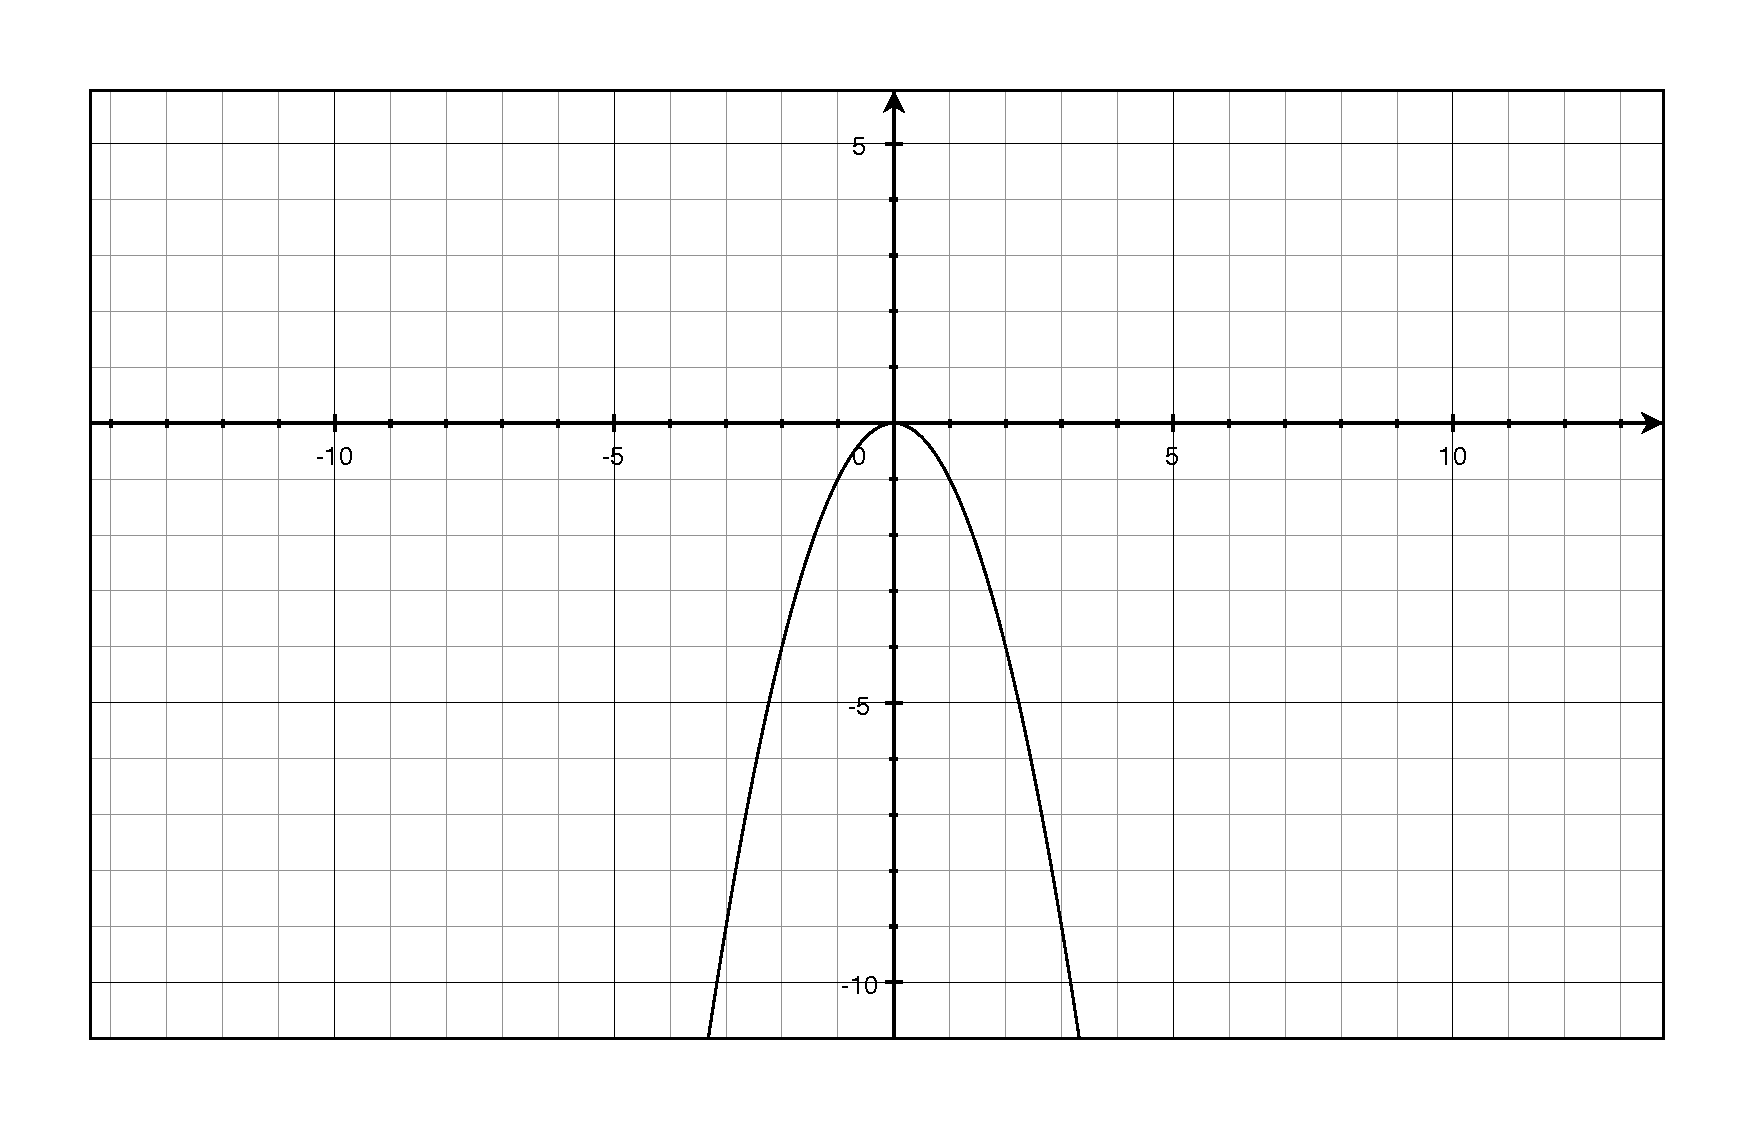
\includegraphics[scale=0.9]{problem7.eps}
%   \caption*{Problem 7}
% \end{figure}

% \begin{tabular}{cc}
%   \toprule
%   period & amplitude \\
%   \midrule
%   value one & value two
%   \bottomrule
% \end{tabular}

\printanswers

\ifprintanswers 
  \usepackage{2in1, lscape} 
\fi

\date{June 17, 2013}
\author{}
\title{Math 141 \\ Homework 15}

\begin{document}

  \maketitle

  \section{Homework}

  Section 4.3: TO DO

 \section{Extra Credit}
  Section 4.3: 61 and 67

  \ifprintanswers
    \begin{description}
      \item[61]
        \begin{align*}
          - \log(x - \sqrt{x^2 - 1}) &= \log(x - \sqrt{x^2 - 1})^{-1} \\
                                     &= \log \frac{1}{x - \sqrt{x^2 - 1}} \\
                                     &= \log \left[ \frac{1}{x - \sqrt{x^2 - 1}} \cdot \frac{x + \sqrt{x^2 - 1}}{x + \sqrt{x^2 - 1}} \right] \\
                                     &= \log \left[ \frac{x + \sqrt{x^2 - 1}}{x^2 - (x^2 - 1)} \right] \\
                                     &= \log ( x + \sqrt{x^2 - 1} ) \\
        \end{align*}

      \item[67]
        The problem is in the last step.  The log of a number less than one is a negative number so the inequality should go the other direction.

    \end{description}
  \fi

  \section{Review}

  \begin{enumerate}

    \item $f(x) = x^3 - 1$ 

  \end{enumerate}

  \ifprintanswers
    \section{Section 4.3}

    \begin{description}

      \item[1] 
        \begin{align*}
          \log_3 \sqrt{27} &= \log_3 27^{1/2} \\
                           &= \frac{1}{2} \log_3 27 \\
                           &= \boxed{\frac{3}{2}} \\
        \end{align*}

      \item[2] 
        \begin{align*}
          \log_2 160 - \log_2 5 &= \log_2 \frac{160}{5} \\
                                &= \log_2 32 \\
                                &= \boxed{5} \\
        \end{align*}

      \item[3] 
        \begin{align*}
          \log 4 + \log 25 &= \log 100 \\
                           &= \boxed{2} \\
        \end{align*}

      \item[4] 
        \begin{align*}
          \log \frac{1}{\sqrt{1000}} &= \log \left( 10^3 \right)^{-1/2} \\
                                     &= - \frac{1}{2} \log 10^3 \\
                                     &= \boxed{-\frac{3}{2}} \\
        \end{align*}

      \item[5] 
        \begin{align*}
          \log_4 192 - \log_4 3 &= \log_4 \frac{192}{3} \\
                                &= \log_4 63 \\
                                &= \boxed{3} \\
        \end{align*}

      \item[6] 
        \begin{align*}
          \log_{12} 9 + \log_{12} 16 &= \log_{12} 144 \\
                                     &= \boxed{2} \\
        \end{align*}

      \item[7] 
        \begin{align*}
          \log_2 6 - \log_2 15 + \log_2 20 &= \log_2 \frac{6 \cdot 20}{15} \\
                                           &= \log_2 8 \\
                                           &= \boxed{3} \\
        \end{align*}

      \item[8] 
        \begin{align*}
          \log_3 100 - \log_3 18 - \log_3 50 &= \log_3 \frac{1}{9} \\
                                             &= \boxed{-2} \\
        \end{align*}

      \item[9] 
        \begin{align*}
          \log_4 16^{100} &= 100 \log_4 16 \\
                          &= \boxed{200} \\
        \end{align*}

      \item[10] 
        \begin{align*}
          \log_2 8^{33} &= 33 \log_2 8 \\
                        &= \boxed{99} \\
        \end{align*}

      \item[11] 
        \begin{align*}
          \log \left( \log 10^{10,000} \right) &= \log 10,000 \\
                                               &= \boxed{4} \\
        \end{align*}

      \item[12] 
        \begin{align*}
          \ln \left( \ln e^{e^{200}} \right) &= \ln \left( e^{200} \right) \\
                                             &= \boxed{200} \\
        \end{align*}

      % \item[13] 
      %   \begin{align*}
      %     \log_2 \left( 2x \right) &= \log_2 2 + \log_2 x \\
      %                              &= \boxed{1 + \log_2 x} \\
      %   \end{align*}

      % \item[14] 
      %   \begin{align*}
      %     \log_3 \left( 5y \right) &= \log_3 5 + \log_3 y \\
      %                              &= \boxed{1 + \log_3 y} \\
      %   \end{align*}

      \item[15] 
        \begin{align*}
          \log_2 (x (x - 1)) &= \boxed{\log_2 x + \log_2 (x - 1)} \\
        \end{align*}

      \item[16] 
        \begin{align*}
          \log_5 \frac{x}{2} &= \boxed{\log_5 x - \log_5 2} \\
        \end{align*}

      \item[17] 
        \begin{align*}
          \log 6^{10} &= \boxed{10 \log 6} \\
        \end{align*}

      \item[18] 
        \begin{align*}
          \ln \sqrt{z} &= \ln z^{1/2} \\
                       &= \boxed{\frac{1}{2} \ln z} \\
        \end{align*}

      \item[19] 
        \begin{align*}
          \log_2 \left( AB^2 \right) &= \log_2 A + \log_2 B^2 \\
                                     &= \boxed{\log_2 A + 2 \log_2 B} \\
        \end{align*}
      \item[20] 
        \begin{align*}
          \log_6 \sqrt[4]{17} &= \log_6 \left( 17^{1/4} \right) \\
                              &= \boxed{\frac{1}{4} \log_6 17} \\
        \end{align*}

      \item[21] 
        \begin{align*}
          \log_3 \left( x \sqrt{y} \right) &= \log_3 x + \log_3 \sqrt{y} \\
                                           &= \log_3 x + \log_3 y^{1/2} \\
                                           &= \boxed{\log_3 x + \frac{1}{2} \log_3 y} \\
        \end{align*}

      \item[22] 
        \begin{align*}
          \log_2 (xy)^{10} &= 10 \log_2 (xy) \\
                           &= \boxed{10 (\log_2 x + \log_2 y)} \\
        \end{align*}

      \item[23] 
        \begin{align*}
          \log_5 \sqrt[3]{x^2 + 1} &= \log_5 \left( x^2 + 1 \right)^{1/3} \\
                                   &= \boxed{\frac{1}{3} \log_5 \left( x^2 + 1 \right)} \\
        \end{align*}

      \item[24] 
        \begin{align*}
          \log_a \left( \frac{x^2}{yz^3} \right) &= \log_a x^2 - \log_a \left( yz^3 \right) \\
                                                 &= 2 \log_a x - \left( \log_a y + \log_a z^3 \right) \\
                                                 &= \boxed{2 \log_a x - \log_a y - 3 \log_a z} \\
        \end{align*}

      % \item[25] 
      %   \begin{align*}
      %     \ln \sqrt{ab} &= \ln (ab)^{1/2} \\
      %                   &= \frac{1}{2} \ln (ab) \\
      %                   &= \boxed{\frac{1}{2} (\ln a + \ln b)} \\
      %   \end{align*}

      % \item[26] 
      %   \begin{align*}
      %     \ln \sqrt[3]{3 r^2 s} &= \frac{1}{3} \ln \left( 3r^2s \right) \\
      %                           &= \frac{1}{3} \left( \ln 3 + \ln r^2 + \ln s \right) \\
      %                           &= \frac{1}{3} \left( \ln 3 + 2 \ln r + \ln s \right) \\
      %   \end{align*}

      % \item[27] 
      %   \begin{align*}
      %     \log \left( \frac{x^3y^4}{z^6} \right) &= \log x^3y^4 - \log z^6 \\
      %                                            &= \log x^3 + \log y^4 - 6 \log z \\
      %                                            &= \boxed{3 \log x + 4 \log y - 6 \log z} \\
      %   \end{align*}

      % \item[28] 
      %   \begin{align*}
      %     \log \left( \frac{a^2}{b^4 \sqrt{c}} \right) &= \log a^2 - \log b^4 c^{1/2} \\
      %                                                  &= \log a^2 - \left( \log b^4 + \log c^{1/2} \right) \\
      %                                                  &= \boxed{2 \log a - 4 \log b + \frac{1}{2} \log c} \\
      %   \end{align*}

      % \item[29] 
      %   \begin{align*}
      %     \log_2 \left( \frac{x \left( x^2 + 1 \right)}{\sqrt{x^2 - 1}} \right)
      %       &= \log_2 \left( x \left( x^2 + 1 \right) \right) - \frac{1}{2} \log_2 \left( x^2 - 1 \right) \\
      %       &= \boxed{\log_2 x + \log_2 \left( x^2 + 1 \right) - \frac{1}{2} \log_2 \left( x^2 - 1 \right)} \\
      %   \end{align*}

      % \item[30] 
      %   \begin{align*}
      %     \log_5 \sqrt{ \frac{x - 1}{x + 1}} &= \frac{1}{2} \log_5 \left( \frac{x - 1}{x + 1} \right) \\
      %                                        &= \boxed{\frac{1}{2} \left( \log_5 (x - 1) - \log_5 (x + 1) \right)} \\
      %   \end{align*}

      \item[31] 
        \begin{align*}
          \ln \left( x \sqrt{ \frac{y}{z}} \right) &= \ln x + \ln \sqrt{ \frac{y}{z}} \\
                                                   &= \ln x + \frac{1}{2} \ln \frac{y}{z} \\
                                                   &= \boxed{\ln x + \frac{1}{2} (\ln y - \ln z)} \\
        \end{align*}

      \item[32] 
        \begin{align*}
          \ln \frac{3x^2}{(x + 1)^{10}} &= \ln \left( 3x^2 \right) - \ln (x + 1)^{10} \\
                                        &= \ln 3 + \ln x^2 - 10 \ln (x + 1) \\
                                        &= \boxed{\ln 3 + 2 \ln x - 10 \ln (x + 1)} \\
        \end{align*}

      \item[33] 
        \begin{align*}
          \log \sqrt[4]{x^2 + y^2} &= \boxed{\frac{1}{4} \log \left( x^2 + y^2 \right)} \\
        \end{align*}

      \item[34] 
        \begin{align*}
          \log \left( \frac{x} {\sqrt[3]{1 - x}} \right) &= \log x - \log (1 - x)^{1/3} \\
                                                         &= \boxed{\log x - \frac{1}{3} \log (1 - x)} \\
        \end{align*}

      \item[35] 
        \begin{align*}
          \log & \sqrt{ \frac{x^2 + 4}{( x^2 + 1 ) ( x^3 - 7 )^2}}  \\
               &= \frac{1}{2} \log \frac{x^2 + 4}{( x^2 + 1 ) ( x^3 - 7 )^2} \\
               &= \frac{1}{2} \left[ \log ( x^2 + 4 ) - \log (  ( x^2 + 1 ) ( x^3 - 7 )^2 ) \right] \\
               &= \frac{1}{2} \left[ \log ( x^2 + 4 ) - (\log ( x^2 + 1 ) + \log ( x^3 - 7 )^2 ) \right]  \\
               &= \boxed{\frac{1}{2} \left[ \log ( x^2 + 4 ) - \log ( x^2 + 1 ) - 2 \log ( x^3 - 7 ) \right]} \\
        \end{align*}

      \item[36] 
        \begin{align*}
          \log \sqrt{x \sqrt{y \sqrt{z}}} &= \log (x (y z^{1/2})^{1/2})^{1/2} \\
                                          &= \log x^{1/2}y^{1/4}z^{1/8} \\
                                          &= \log x^{1/2} + \log y^{1/4} + \log z^{1/8} \\
                                          &= \boxed{\frac{1}{2} \log x + \frac{1}{4} \log y + \frac{1}{8} \log z}  \\
        \end{align*}

      \item[37] 
        \begin{align*}
          \ln \left( \frac{x^3 \sqrt{x - 1}}{3x + 4} \right) &= \ln (x^3 \sqrt{x - 1}) - \ln (3x + 4) \\
                                                             &= \boxed{3 \ln x + \frac{1}{2} \ln (x - 1) - \ln (3x + 4)} \\
        \end{align*}

      \item[38] 
        \begin{align*}
          \log & \left( \frac{10^x}{x(x^2 - 1)(x^4 + 2)} \right) = \log 10^x - \log (x(x^2 - 1)(x^4 + 2)) \\
                                                               &= x - ( \log x + \log (x^2 - 1) + \log (x^4 + 2)) \\
                                                               &= \boxed{x - \log x - \log (x^2 - 1) - \log (x^4 + 2)} \\
        \end{align*}

      \item[39] 
        \begin{align*}
          \log_3 5 + 5 \log_3 2 &= \log_3 5 + \log_3 2^5 \\
                                &= \log_3 (5 \cdot 2^5) \\
                                &= \boxed{\log_3 160} \\
        \end{align*}

      \item[40] 
        \begin{align*}
          \log 12 + \frac{1}{2} \log 7 - \log 2 &= \log 12 + \log 7^{1/2} - \log 2 \\
                                                &= \log \frac{12 \sqrt{7}}{2} \\
                                                &= \boxed{\log (6 \sqrt{7})} \\
        \end{align*}

      \item[41] 
        \begin{align*}
          \log_2 A + \log_2 B - 2 \log_2 C &= \log_2 A + \log_2 B - \log_2 C^2 \\
                                           &= \boxed{\log_2 \frac{AB}{C^2}} \\
        \end{align*}

      \item[42] 
        \begin{align*}
          \log_5 (x^2 - 1) - \log_5 (x - 1) &= \log_5 \frac{x^2 - 1}{x - 1} \\
                                            &= \log_5 \frac{(x + 1)(x - 1)}{x - 1} \\
                                            &= \boxed{\log_5 (x + 1)} \\
        \end{align*}

      \item[43] 
        \begin{align*}
          4 \log x &- \frac{1}{3} \log (x^2 + 1) + 2 \log (x - 1) \\
                   &= \log x^4 - \log (x^2 + 1)^{1/3} + \log (x - 1)^2 \\
                   &= \boxed{\log \frac{x^4 (x - 1)^2}{(x^2 + 1)^{1/3}}} \\
        \end{align*}

      \item[44] 
        \begin{align*}
          \ln(a + b) + \ln(a - b) - 2 \ln c &= \ln(a + b) + \ln(a - b) - \ln c^2 \\
                                            &= \ln \frac{(a + b)(a - b)}{c^2} \\
                                            &= \boxed{\ln \frac{a^2 - b^2}{c^2}} \\
        \end{align*}

      \item[45] 
        \begin{align*}
          \ln 5 + 2 \ln x + 3 \ln (x^2 + 5) &= \ln 5 + \ln x^2 + \ln (x^2 + 5)^3 \\
                                            &= \boxed{\ln \left[ 5x^2 (x^2 + 5)^3 \right]} \\
        \end{align*}

      \item[48] 
        \begin{align*}
          \log_a b + c \log_a d - r \log_a s &= \log_a b + \log_a d^c - \log_a s^r \\
                                             &= \boxed{\log_a \frac{bd^c}{s^r}} \\
        \end{align*}

      \item[49] 
        \begin{align*}
          \log_2 5 &= \frac{\ln 5}{\ln 2} \\
                   &\approx \boxed{2.32193} \\
        \end{align*}

      \item[50] 
        \begin{align*}
          \log_5 2 &= \frac{\ln 2}{\ln 5} \\
                   &\approx \boxed{0.430677} \\
        \end{align*}

      \item[51] 
        \begin{align*}
          \log_3 16 &= \frac{\ln 16}{\ln 3} \\
                   &\approx \boxed{2.52372} \\
        \end{align*}

      \item[52] 
        \begin{align*}
          \log_6 92 &= \frac{\ln 92}{\ln 6} \\
                   &\approx \boxed{\boxed{2.52366}} \\
        \end{align*}

      \item[59] 
        \begin{align*}
          \log e &= \frac{\ln e}{\ln 10} \\
                 &= \boxed{\frac{1}{\ln 10}} \\
        \end{align*}

      \item[60] 
        \begin{align*}
          (\log_2) (\log_5 7) &= \frac{\ln 5}{\ln 2} \cdot \frac{\ln 7}{\ln 5} \\
                              &= \boxed{\frac{\ln 7}{\ln 2}} \\
        \end{align*}

      \item[63]
        \begin{enumerate}[a]
          \item 
            \begin{align*}
              \log P &= \log c - k \log W \\
                     &= \log c - \log W^k \\
                     &= \log \frac{c}{W^k} \\
                   P &= \boxed{\frac{c}{W^k}} \\
            \end{align*}

          \item
            \begin{align*}
              P(2)  & = \frac{8,000}{2^{2.1}} \\
                    & \approx \boxed{\unit[1,866]{people}} \\
              \\
              P(10) & = \frac{8,000}{10^{2.1}} \\
                    & \approx \boxed{\unit[64]{people}} \\
            \end{align*}

        \end{enumerate}

      \item[64]
        \begin{enumerate}[a]
          \item 
            \begin{align*}
              \log S &= \log c + k \log A \\
                     &= \log c + \log A^k \\
                     &= \log cA^k \\
                   S &= \boxed{cA^k} \\
            \end{align*}

          \item
            \begin{align*}
              S     &= cA^3 \\
              S(2A) &= c (2A)^3 \\
                    &= 8 cA^3 \\
                    &= \boxed{8 S(A)} \\
            \end{align*}

        \end{enumerate}


    \end{description}

  \else
    \vspace{2 cm}
    \begin{quote}
      \begin{em}
        TO DO
      \end{em}
    \end{quote}

    \hspace{1 cm} --Carl Jung
  \fi

\end{document}

